In the upcoming chapter, we discuss the methodology of $\emph{Translucify}$ in detail. We begin with a general framework overview and discuss the specific approaches individually.

\section{Framework Overview}
In order to look deeper into the main problem of this thesis, we first formally define our problem as described below.

\begin{definition}[Translucent Log Extension Problem]
\label{def:tlgp}
    Given an event log $\mathcal{L} \subseteq \mathcal{E}$ as input, produce a translucent event log $\mathcal{L'}$ where the set of enabled activities are added as attributes. 
\end{definition}

There is a variant of the \emph{Translucent Log Extension Problem}, where a process model is provided along with the event log.

\begin{definition}[Translucent Log Extension Problem - Process Model Variant]
\label{def:tlgpm}
    Given an event log $\mathcal{L}$ and a process model $\mathcal{M}$ as inputs, produce a translucent event log $\mathcal{L'}$ where the set of enabled activities are added as attributes. 
\end{definition}

The second variant differs from the first, as the model is meant to act as a reference model; the set of enabled activities is intended to be constrained by the process model. Note that the function of $\mathcal{M}$ is to provide an upper bound on the set of enabled activities, and the log is there to provide further constraints to enrich the model. Of particular interest are parallel and choice situations, since we are able to deduce supplementary patterns not demonstrated in the process model using log data. We name the first variant defined in Definition \ref{def:tlgp} as \emph{Bottom-up Translucent Log Extension Problem}, whereas the second variant in Definition \ref{def:tlgpm} is named as \emph{Top-down Translucent Log Extension Problem.}


\begin{table}[h]
    \centering
	\caption{A table of available model-based options for \emph{Translucify}.}
    \begin{tabular}{|c|c|c|}
        \hline
        & \textbf{Petri Net} & \textbf{Prefix Automaton} \\ 
        \hline
        \textbf{Logistic Regression} & LR with Petri nets & LR with prefix automata \\
        \hline
        \textbf{Random Forests} & RF with Petri nets & RF with prefix automata \\
        \hline
    \end{tabular}
    \label{tab:framework_overview}
\end{table}

\section{Petri Net-based Approaches} \label{sec:petri_net_approaches}

The basic notion of Petri nets was introduced in the previous \cref{chap:prelim}. In this section, we will discuss how Petri nets are employed to tackle the \emph{Translucent Log Extension Problem}.

\begin{figure}
    \centering
    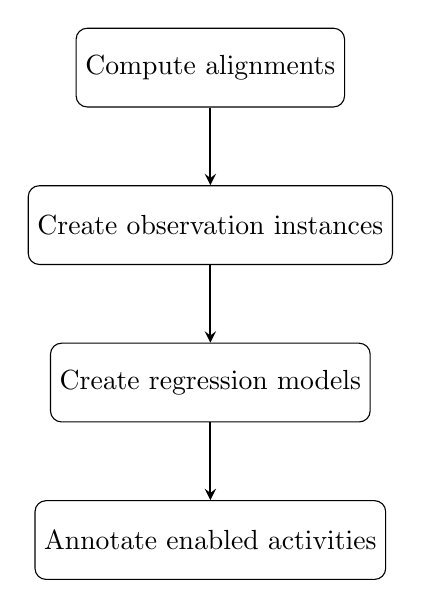
\begin{tikzpicture}[node distance=2cm, auto]
        % Define block styles
        \tikzstyle{stage} = [rectangle, rounded corners, minimum width=3cm, minimum height=1cm, text centered, draw=black]
        \tikzstyle{arrow} = [thick,->,>=stealth]
        
        % Nodes
        \node (stage1) [stage] {Compute alignments};
        \node (stage2) [stage, below of=stage1] {Create observation instances};
        \node (stage3) [stage, below of=stage2] {Create regression models};
        \node (stage4) [stage, below of=stage3] {Annotate enabled activities};
        
        % Arrows
        \draw [arrow] (stage1) -- (stage2);
        \draw [arrow] (stage2) -- (stage3);
        \draw [arrow] (stage3) -- (stage4);
    \end{tikzpicture}
    \caption{Stages of multivariable regression on an SLDPN.}
    \label{sldpn-multivar-regression}
\end{figure}

Given a Petri net and an event log, we utiltize the alignment-based appraoch presented in \cite{creating-translucent-event-logs} as its baseline algorithm. After computing the alignment for each trace, the program replays the alignment on the reachabiliy graph trace by trace in order to circumvent the silent transitions. For each activity, the algorithm then augments the event log with the corresponding transitions situated in outgoing arcs of the current state. After creating a basic translucent event log, the log can be refined by further algorithms.

\dots

When annotating the event log with enabled activities, it might make sense to assume that not all activities enabled in the model are enabled in reality. The model might be too permissive to guarantee its fitness to the event log, and the set of enabled activities depicted in the model should therefore be considered as an upper bound of the actual set. Here, instead of applying a hard-line policy by adding guards to the transitions as done in the field of decision mining, we can utilize a probabilistic approach to filter out the activities. An important question would be how we should compute the transition probability of the model. This is where the SLDPN model comes into play.

A method to incorporate the data attributes is to implement multivariable regression. Similar to the setting in \cite{sldpn}, we construct a training data set for each transition of a Petri net consisting of data attributes and a boolean label indicating whether the transition was executed given the data attributes as input. We then perform a regression analysis on the training data set for each transition. The resulting dictionary of transitions and regression functions can be employed to filter out transitions lying below a certain probability threshold $p$ in each decision point during replay.

\begin{figure}
    \centering
    \begin{tikzpicture}[place/.style={circle, draw, minimum size=6mm}, transition/.style={rectangle, draw, minimum width=8mm, minimum height=8mm}, every edge/.style={draw, thick}]
        % Places
        \node[place] (p1) at (0, 0) {};
        \node[place] (p2) at (4, 0) {};
        \node[place] (p3) at (8, 0) {};
        \node[place] (p4) at (12, 0) {};
        
        % Transitions
        \node[transition] (a) at (2, 0) {a};
        \node[transition] (b) at (6, 2) {b};
        \node[transition] (t1) at (6, 0) {$\tau$};
        \node[transition] (c) at (6, -2) {c};
        \node[transition] (d) at (10, 0) {d};

        % Make tau transitions black!

        
        % Arcs
        \draw[->] (p1) -- (a);
        \draw[->] (a) -- (p2);
        
        \draw[->] (p2) -- (b);
        \draw[->] (p2) -- (t1);
        \draw[->] (p2) -- (c);
        
        \draw[->] (b) -- (p3);
        \draw[->] (t1) -- (p3);
        \draw[->] (c) -- (p3);

        \draw[->] (p3) -- (d);
        \draw[->] (d) -- (p4);
    \end{tikzpicture}
    \caption{Example Petri net for multivariable regression.}
    \label{fig:model-multivar-regression}
\end{figure}


\begin{table}[h]
    \centering
    \caption{Example event log for multivariable regression.}
    \begin{tabular}{|c|c|c|c|c|}
    \hline
    Case ID & Activity & Timestamp & Family History & Amount \\
    \hline
    101 & a & 2024-08-01 08:00:00 & yes & 30 \\
    101 & d & 2024-08-01 08:30:00 & yes & 50 \\
    102 & a & 2024-08-02 09:00:00 & no & 0 \\
    102 & b & 2024-08-02 09:45:00 & no & 40 \\
    102 & d & 2024-08-02 10:30:00 & no & 56 \\
    \hline
    \end{tabular}
    \label{tab:log-multivar-regression}
    \end{table}
\subsubsection*{Computing Alignments}

A process model does not always guarantee a perfect fitness of the event log. Sometimes, infrequent traces are considered as noise and are subsequently ignored. Furthermore, process models contain more than one unique fitting path for each trace in various occasions. It is therefore crucial in Petri nets to first compute the best-fitting model trace for each log trace using \emph{alignments} \cite{alignments}.

(theoretical background \& explanation on how alignments usually work)

Computing alignments can be thought as choosing an alignment function $f_{align} \colon \mathcal{L} \rightarrow T^*$, where given a log trace $\sigma \in \mathcal{L}$ as input, $f_{align}$ returns a sequence of transitions $\langle t_1, \dots, t_n \rangle$ as output, corresponding to the optimal model trace computed by a chosen alignment algorithm.

In our scenario, however, we need to take data attributes into account as well, which are necessary for the regression analysis. For this, the appropriate data attributes of the log trace must be attached to the model trace. Intuitively, since event logs are records of a system, we assume that the data state is the data snapshot immediately after the event occurrence. Moreover, we assume that silent transitions do not modify the data state. Data states of silent transitions in the model trace are therefore identical to the most recently occurred data state of a named transition recorded in the event log.

We therefore extend the alignment function to $f_{align} \colon \mathcal{L} \rightarrow (T \times \Delta)^*$, where $\Delta$ is the set of data attributes found in the corresponding event $e \in \sigma$. Given a log trace $\sigma \in \mathcal{L}$ and the corresponding data attributes $d \in \Delta$, $f_{align}(\sigma) = \langle (t_1, d_1), \dots, (t_n, d_n) \rangle$ returns a sequence of transitions as output.

Using the example event log in Table \ref{tab:log-multivar-regression} and the model in Figure \ref{fig:model-multivar-regression}, the alignment for the trace $\langle a, d \rangle$ would be $((a, (yes, 30)), (t1, (yes, 30)), (d, (yes, 50)))$, and the alignment for trace $\langle a, b, d \rangle$ would be $((a, (no, 0)), (b, (no, 40)), (d, (no, 56)))$.

\subsubsection*{Creating Observation Instances}

Given an aligned model trace, our goal is to generate a labeled training data set for each transition in the Petri net model. In other words, the goal of this stage is to find the function $f_{observe} \colon T \rightarrow (\Delta \times \{0, 1\})^*$.

We iterate over the event log and replay the Petri net using the model trace $f_{align}(\sigma)$ $\forall \sigma \in \mathcal{L}$. For each Petri net marking $M_i$ where $(N, M_0)[\langle t_1, \dots, t_{i-1} \rangle \rangle (N, M_i)$ and the corresponding current data state $d_i$, we first compute the enabled transitions $en(M_i)$ and update the values of $f_{observe}$ as the following:
$f_{observe}(t_j) \leftarrow f_{observe}(t_j) \cup \{ (d_i, c)\}$ for all $t_j \in en(M_i)$, where

\[
    c =
    \begin{cases}
        1 & \text{if } t_i = t_j\\
        0 & \text{otherwise.}
    \end{cases}
\]

Looking at our running example, the observation instance function $f_{observe}$ would be as follows:

\[
    f \colon t \mapsto
    \begin{cases}
        \Bigl[((yes, 30), 1), ((no, 0), 1) \Bigr], & t = a\\
        \Bigl[((yes, 30), 0), ((no, 0), 1)\Bigr], & t = b\\
        \Bigl[((yes, 30), 0), ((no, 0), 0)\Bigr], & t = c\\
        \Bigl[ ((yes, 30), 1), ((no, 40), 1)\Bigr], & t = d\\
    \end{cases}
\]

\subsubsection*{Create regression models}

After creating the observation instances, we train a logistic regression model for each transition in the Petri net model. The goal of this stage is to find the function $f_{regress} \colon T \times \Delta \rightarrow [0 , 1]$, which returns the probability of a transition being enabled given the data attributes.

\subsubsection*{Annotating the log with enabled activities}

After training a logistic regression model for each transition, the goal of this stage is to utilize the regression functions and the alignments to add enabled activities to events listed in each trace. In other words, we need to compute a function $f_{annotate} \colon \mathcal{L} \times [0, 1] \rightarrow \mathcal{L'}$, where given a log trace $\sigma \in \mathcal{L}$ and a threshold $t \in [0, 1]$, $f_{annotate}$ returns a translucent trace $\sigma'$ where $\pi_{en}(e) \in \mathcal{P(\mathcal{A})}$ for all trace events $e \in \sigma$.

\section{Random Forest-based Approaches}

We do the same thing as above, but instead of using logistic regression, we use random forests.

\section{Transition System-based Approaches}

In this section, we discuss how transition systems, in particular prefix automata, can be exploited as an additional process model for the \emph{Translucent Log Extension Problem}.

One of the advantages of utilizing transition systems over Petri nets is the lack of silent transitions. When trying to replay a trace on a Petri net in the presence of silent transition, the algorithm must decide which path of the firing sequence it should take by computing alignments with a certain cost function, then taking the path with the minimal cost. This can be computationally expensive and time-consuming, especially for larger models where the number of silent transitions is high. Transition systems can benefit us in this regard.

\subsection{Frequency-Annotated Prefix Automata}

\begin{definition}[Frequency-Annotated Prefix Automaton]
    Let $\mathcal{L} \subseteq \mathcal{E}$ be a simple event log. A \emph{Frequency-Annotated Prefix Automaton (FAPA)} is a tuple $\mathit{PA}_{freq} = (S, A, T, f)$, where $(S, A, T)$ is a prefix automaton $\mathit{TS}_{L, hd}$ following the Definition \ref{def:pa} and  $f \colon S \to \mathbb{N}, \sigma_{pref} \mapsto \lvert \{ \sigma \in \mathcal{L} \mid \sigma_{pref} \sqsubseteq \sigma \}\rvert$ is a frequency labeling function.
\end{definition}

Let us look at a small example. Consider the simple event log $\mathcal{L} = [\langle a, b, c \rangle^{30}, \langle a, b, d \rangle^{10}]$. The resulting FAPA is depicted in \ref{fig:fapa}. The frequency labeling function $f$ is represented as in the usual superscript notation used in trace multiset of simple event logs.

% \begin{algorithm}
% \caption[short]{FAPA Generation}
%     \For{$\sigma \in \mathcal{L}$}
%     {
%         \For{$i \in \lvert \sigma \rvert$}
%         {
%             $\sigma_{pref} \gets hd_i(\sigma)$\;
%             $f(\sigma) \gets f(\sigma) + 1$\;
%         }
%     }
% \end{algorithm}

\begin{figure}[H]
    \centering
    \begin{tikzpicture}[auto, node distance=3cm, 
        every node/.style={draw, ellipse, font=\sffamily\large\bfseries, inner sep=1pt, outer sep=0pt, minimum height=1cm},
        every edge/.style={draw, -{Stealth[]}, thick}]

        \node (1) {$\langle \rangle^{40}$};
        \node (2) [right of=1] {$\langle a \rangle^{40}$};
        \node (3) [right of=2] {$\langle a, b \rangle^{40}$};
        \node (4) [above right of=3] {$\langle a, b, c \rangle^{30}$};
        \node (5) [below right of=3] {$\langle a, b, d \rangle^{10}$};

        \path[every node/.style={font=\sffamily\small}]
        (1) edge node {a} (2)
        (2) edge node {b} (3)
        (3) edge node {c} (4)
        edge node {d} (5);
    \end{tikzpicture}
    \caption{Resulting FAPA from $\mathcal{L}$.}
    \label{fig:fapa}
\end{figure}

Given a certain threshold, a simple algorithm would be to iterate over each trace in the event log and annotating the enabled activities with transitions lying above the threshold. For an example threshold value of $t = 0.5$, the resulting simple translucent event log would be: $[\langle \underline{a}, \underline{b}, \underline{c} \rangle^{30}, \langle \underline{a}, \underline{b}, c\underline{d}\rangle^{10}]$. Note that annotating enabled activities using conventional prefix automata can be considered as a special case of this problem with threshold $t = 0$.

\subsection{Merging States}

As discussed in the previous \cref{subsec:transition_systems}, list-based prefix automata can precisely describe the behavior of an event log, but it fails at creating a generalized process model due to its inability of recognizing loops and parallel behavior.

In order to overcome this issue, we introduce a merge operator for the list-based prefix automata. The merge operator is defined as the following:

\begin{definition}[State Merging]
    Let $PA = (S, A, T, f)$ be a prefix automaton. A \emph{State-merged prefix automaton} of $PA$ is a prefix automaton $PA_{\Yright} = (S_{\Yright}, A_{\Yright}, T_{\Yright}, f_{\Yright})$, where $S' \subseteq \mathcal{P}(S), A_{\Yright} = A,  T' \subseteq S' \times A \times S'$, and $f_{\Yright} = f$.

    Let $s_1, s_2 \in S_{\Yright}$ be two distinct states of a state-merged prefix automaton. $ PA_{\Yright} \underset{s_1, s_2}{\rightpitchfork} PA_{\Yright}'$ denotes that the state merge operator $\rightpitchfork$ applied on a state-merged prefix automaton $PA_{\Yright}'$ together with states $s_1, s_2$ returns a new state-merged prefix automaton $PA_{\Yright}' = (S_{\Yright}', A_{\Yright}', T_{\Yright}', f_{\Yright}')$ with following properties:

    \begin{itemize}
        \item $S_{\Yright}' = ( S_{\Yright} / \{s_1, s_2\} ) \cup s'$, where $s'$ is a new state with $s' = s_1 \cup s_2$.
        \item $A_{\Yright}' = A_{\Yright}$.
        % Remove all transitions that have $s_1$ or $s_2$ as source or target state and add new transitions with $s'$ as source or target state.
        \item $T_{\Yright}' = (T_{\Yright} / \{ (s_{\alpha}, a, s_{\beta}) \mid a \in A_{\Yright}, s_{\alpha} \in \{s_1, s_2 \} \lor s_{\beta} \in \{s_1, s_2\} \}) \cup \{ (s', a, s) \mid (s_1, a, s) \in T_{\Yright} \lor (s_2, a, s) \in T_{\Yright} \} \cup \{ (s, a, s') \mid (s, a, s_1) \in T_{\Yright} \lor (s, a, s_2) \in T_{\Yright} \}$.
        \item $f_{\Yright}' = f_{\Yright}$.
    \end{itemize}    
\end{definition}

Using the previous prefix automaton in Figure \ref{fig:example_prefix_automaton} as an example, we first create a state-merged prefix automaton as follows in Figure \ref{fig:state_merged_prefix_automaton_0}.

\begin{figure}
    \centering
    \begin{tikzpicture}[->,>=stealth',shorten >=1pt,auto,node distance=2.8cm,
                        semithick]
    \tikzstyle{every state}=[fill=white,draw=black,text=black]
    
    \node[state] (<>) { $\{ \langle \rangle \}$ };
    \node[state] (<a>) [right of=<>] {$\{ \langle a \rangle \}$};
    \node[state] (<ab>) [below right of=<a>] {$\{ \langle a, b \rangle \}$};
    \node[state] (<abc>) [right of=<ab>]       {$\{ \langle a, b, c \rangle \}$};
    \node[state] (<abcd>) [right of=<abc>]       {$\{ \langle a, b, c, d \rangle \}$};
    \node[state] (<ac>) [above right of=<a>]       {$\{ \langle a, c \rangle \}$};
    \node[state] (<acb>) [right of=<ac>]       {$\{ \langle a, c, b \rangle \}$};
    \node[state] (<acbd>) [right of=<acb>]       {$\{ \langle a, c, b, d \rangle \}$};
    
    \path (<>) edge node {a} (<a>)
          (<a>) edge node {b} (<ab>)
          (<a>) edge node {c} (<ac>)
          (<ab>) edge node {c} (<abc>)
          (<ac>) edge node {b} (<acb>)
          (<abc>) edge node {d} (<abcd>)
          (<acb>) edge node {d} (<acbd>);
    \end{tikzpicture}
    \caption{Generated state-merged prefix automaton based on Figure \ref{fig:example_prefix_automaton}.}
    \label{fig:state_merged_prefix_automaton_0}
\end{figure}

After merging the states $\{ \langle a, c, b \rangle \}$ and $\{ \langle a, b, c \rangle \}$, the resulting state-merged prefix automaton is depicted in Figure \ref{fig:state_merged_prefix_automaton_1}. The new state $\{ \langle a, b, c \rangle, \langle a, c, b \rangle \}$ inherits the incoming and outgoing transitions of the merged states.

\begin{figure}[H]
    \centering
    \begin{tikzpicture}[->,>=stealth',shorten >=1pt,auto,node distance=2.8cm, semithick]
    \tikzstyle{every state}=[fill=white,draw=black,text=black]
    
    \node[state] (<>) { $\{ \langle \rangle \}$ };
    \node[state] (<a>) [right of=<>] {$\{ \langle a \rangle \}$};
    \node[state] (<ab>) [below right of=<a>] {$\{ \langle a, b \rangle \}$};
    \node[state, style=ellipse] (<abc>) [above right of=<ab>]       {$\{ \langle a, b, c \rangle, \langle a, c, b \rangle \}$};
    \node[state] (<abcd>) [below right of=<abc>]       {$\{ \langle a, b, c, d \rangle \}$};
    \node[state] (<ac>) [above right of=<a>]       {$\{ \langle a, c \rangle \}$};
    \node[state] (<acbd>) [above right of=<abc>]       {$\{ \langle a, c, b, d \rangle \}$};
    
    \path (<>) edge node {a} (<a>)
          (<a>) edge node {b} (<ab>)
          (<a>) edge node {c} (<ac>)
          (<ab>) edge node {c} (<abc>)
          (<ac>) edge node {b} (<abc>)
          (<abc>) edge node {d} (<abcd>)
          (<abc>) edge node {d} (<acbd>);
    \end{tikzpicture}
    \caption{State-merged prefix automaton after merging states $\{ \langle a, c, b \rangle \}$ and $\{ \langle a, b, c \rangle \}$ together.}
    \label{fig:state_merged_prefix_automaton_1}
\end{figure}

State merging brings two advantages. Firstly, the state space can be significantly reduced depending on the operator's preference. Secondly, behaviors which were previously impossible to capture using conventional prefix automata, such as loops or parallel executions, can now be represented in the state-merged prefix automaton.

After state merging, we can utilize the resulting automaton for multivariate regression in the identical manner as described in the Petri net-based approach in section \ref{sec:petri_net_approaches}.

\section{Transformer-based Approaches}

Buttom-up approaches aims to discover enabled activities without the help of a process model. \dots

A simple approach is to utilize the \emph{directly-follows matrix} of an event log.
Given an event log $\mathcal{L}$, we compute the set of unique activities and generate a next-activity matrix $\mathbf{A}$, where the entry $\mathbf{A}_{ij}$ represents the number of times activity $j$ follows activity $i$. We can then easily transform $\mathbf{A}$ into a probability matrix $\mathbf{A'}$ by dividing each row by the sum of the row. We then filter out the results by a certain threshold $p$ and add the entries surviving the threshold to each event trace. This algorithm can serve as baseline for further extensions. We formally define the directly-follows matrix as follows:

\begin{definition}[Directly-follows Matrix]
    Let $\mathcal{L}$ be an event log. Let further $U = \pi_{act}(L) = \bigcup\limits_{\sigma \in \mathcal{L}} \{ \pi_{act}(e) \mid \pi_{act}(e) \in \sigma \}$ be the set of unique activities in $\mathcal{L}$. $\mathbf{A}$ is a \emph{directly-follows matrix} of $\mathcal{L}$, if:

    \begin{itemize}
        \item $\mathbf{A} \in \mathbb{N}^{n \times n}$ , where $n = \lvert U \rvert$, i.e., the number of unique activities in $\mathcal{L}$.
        
        \item Let $\{ U_j \}_{j \in J}$ be an indexed family of $U$ with $J = \{ 1, 2, \dots, n\}, n = \lvert U \rvert$. $\mathbf{A}_{ij} = \sum\limits_{\sigma \in \mathcal{L}} \Big| \{ i \mid 1 \leq i \leq \lvert \sigma \rvert, \sigma(i) = U_i \land \sigma(i+1) = U_j \} \Big|$, i.e., the absolute frequency activity $U_i$ is directly followed by activity $U_j$.
    \end{itemize}
\end{definition}

Given the directly-follows matrix as a baseline, there are several applications to extend the matrix. One of the most straightforward approaches is transforming the matrix into a Markov matrix.

\begin{definition}[Probabilistic Directly-follows Matrix]
    Let $\mathbf{A = (a_{ij})}$ be a directly-follows matrix of an event log $\mathcal{L}$. $\mathbf{A'} = (a'_{ij})$ is a \emph{probabilistic directly-follows matrix} of $\mathcal{L}$ if

    \[
        a'_{ij} = \frac{a_{ij}}{\sum\limits_{k=1}^{n} a_{ik}}.
    \]

\end{definition}



\begin{itemize}
    
    \item Furthermore, we can utilitze a deep-learning based black-box approach. The issue with implementing supervised learning algorithms is that we need a labeled training dataset. In our case, this would be a preexisting translucent event log, which is unavailable in our setting due to missing enabled activities data. We can cirucmvent the problem by training the model using the next activity information as label, as this information is available in every event log. Since most learning algorithms would not return a single value but an underlying probability distribution of possible outcomes, we can substitute the final $\mathit{argmax}$ operation with selecting a threshold $p$ and returning all labels lying above it.
\end{itemize}



